\chapter{Design}
\label{cha:design}
\textit{The design of WOMBAT has changed throughout the project. The design chapter presents the vision of the timer application and the tools used to design and develop the product.} % Rettet

\section{Vision}
\label{sec:vision}
Since the launcher had both a child-mode and a guardian-mode at the first period of the project, this vision relies on the initial design of the launcher project.\\ \\
	The idea of the WOMBAT application was, that is should be a tool for educators to illustrate time for the children.\\
	
One part is the timer application as it is implemented, from which it is possible to run timers, such as an hourglass or a digital watch. This part should be available only from the guardian-mode.\\ \\
  The second part of the application is a timer overlay, which is launched when other applications are launched through the GIRAF launcher. When such applications are launched through guardian mode, the user should be prompted to select if there is a time limit on the application, and what the limit should be. If a time limit is chosen, the given application, i.e. a game, is run with the timer overlay showing a custom timer with the time left (see figure \ref{fig:init_overlay_drawings}).
	
	\begin{figure}[H]
		\centering
			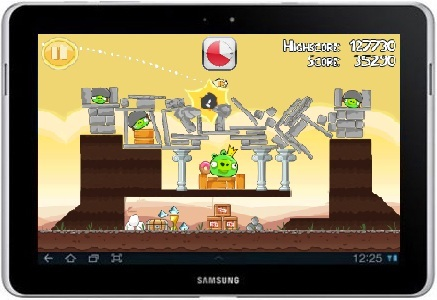
\includegraphics[width=\textwidth]{Images/paper_prototype/overlay.png}
				\caption{Example of how the timer overlay would look. Here there is an overlay on a game with about 40 minutes left.}
		\label{fig:init_overlay_drawings}
	\end{figure}
	
	If the launcher is in child-mode, and the child opens an application, the timer overlay is run according to settings chosen in the third and last part of the WOMBAT system; the settings application. The overlay can be used if a child is only allowed to play a game for 30 minutes a day, then the overlay can be customized to show the child how much time is left of the allowed time. When the time has expired, the application is automatically closed.\\ \\
	The third part of the application is only available from the guardian-mode in the launcher, and from this application it is possible to customize which applications should be run with the timer overlay. Also it is possible to define how the overlay for every child should look like, and what should happen when the time limit has been reached. Also it is also possible to set constrains for the applications, such as time constrains, i.e. certain applications can only be opened in a different timespan on the day, or when a specific application has been run for 30 minutes straight, the application is closed and cannot be opened before a certain "cooldown" has ended.

\section{Stories}
These stories are fictive, and are based on the vision of the timer system, together with an interview with our contact person.\\
We use a fictive person in the use cases, Trine, who acts as an educator in a special kindergarden for children with ASD.

	\subsection*{Timer Application}
	Trine got an Android tablet from the kindergarden yesterday, and some of the other educators suggested that she should try out the WOMBAT timer application. Trine has planned a playing session with a few of the children, and decides to use the WOMBAT application to time the session, such that the children can see when they are done playing. They have about 30 minutes to play in, so Trine opens WOMBAT on the tablet and selects a predefined hourglass set to 30 minutes. When the children are in place and ready to play, she press the start button, and the hourglass starts. When the time runs out, a "Done" screen appear, and the children can see that they are done playing.

	\subsection*{Timer Overlay}
	Trine walks in the playground while the children are playing. She sees one of the boys sitting on the ground in the corner of the playground. She walks over to him. It is Casper, he had tripped over his own feet, and hurt his knee. To get Caspers mind of his knee Trine lets Casper play his favorite computer game for the next 10 minutes. She starts the game, and gets prompted to choose a profile and the amount of time the game should allow to run. She selects Casper's profile and 10 minutes. The game starts with the timer overlay showing 10 minutes left of play time, with Casper's favorite green digital clock. When the time has run out, the game closes, and Casper is again ready to play with his friends.

\section{Prototyping}
Before the actual development started, we made a few drawings of our ideas (see figure \ref{fig:init_drawings}).

	\begin{figure}[H]
		\centering
			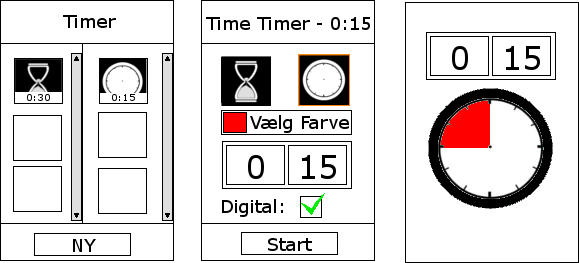
\includegraphics[width=\textwidth]{Images/paper_prototype/init_drawings.png}
				\caption{Drawing of the initial ideas of the timer application.}
		\label{fig:init_drawings}
	\end{figure}

	\subsection*{Paper Prototyping}
	Paper prototypes\cite{misc:designInterSys} has been used in the first iterations in the development process. The initial idea of the system design was drawn on paper, so that our contact person could give us some feedback on the design, before we started programming. In figure \autoref{fig:pap_prot_menu} is a paper prototype of the menu in the timer application, and the rest of the prototypes can be found in appendix \autoref{sec:paper_prot}.

	\begin{figure}[H]
		\centering
			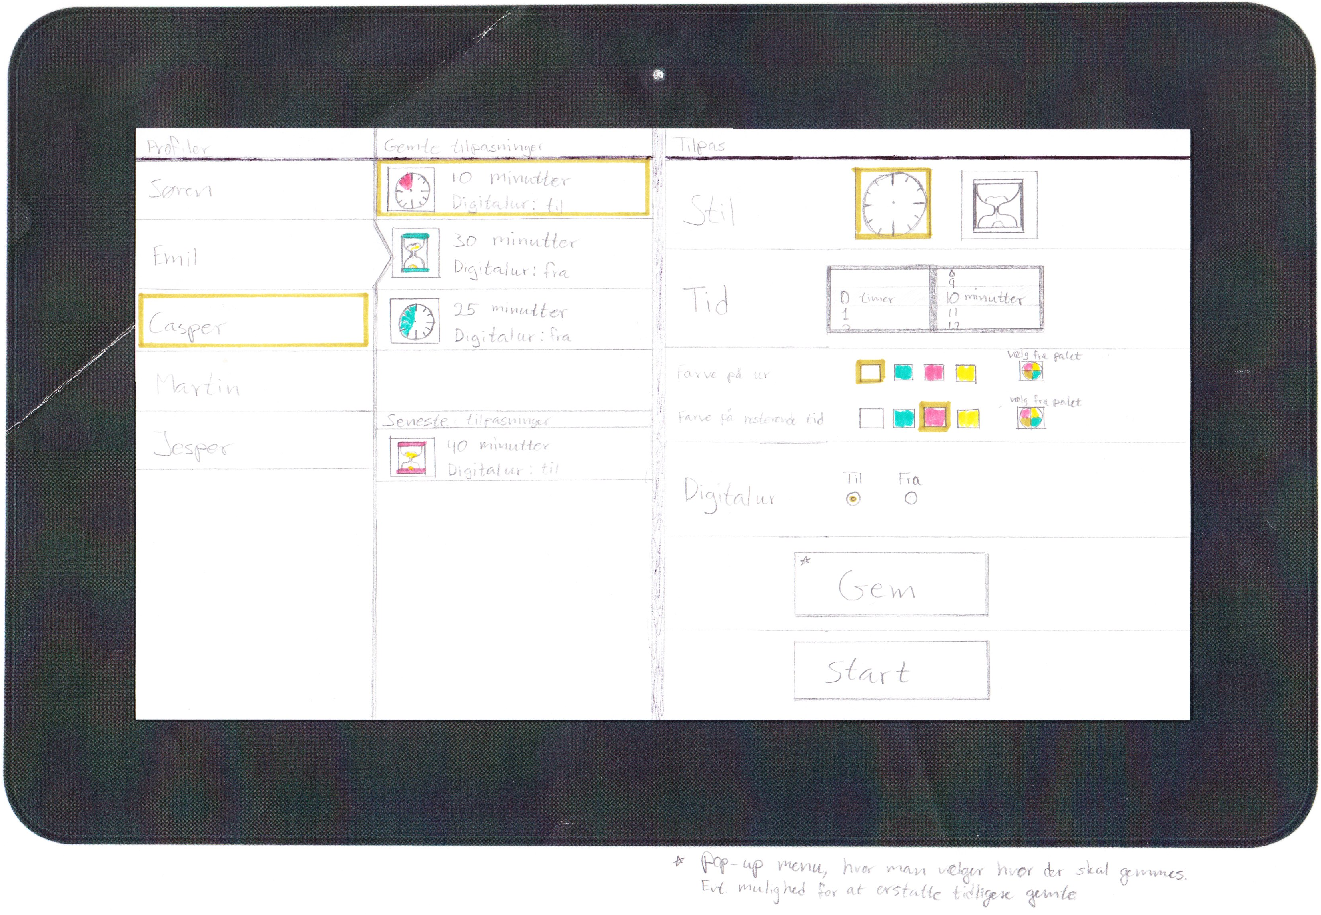
\includegraphics[width=\textwidth]{Images/paper_prototype/menu.png}
				\caption{Scan of a paper prototype of the menu in the timer application.}
		\label{fig:pap_prot_menu}
	\end{figure}

Paper prototypes are produced quickly, and they capture early design ideas.

	\subsection{Metaphors}
	To enhance usability and learn-ability, we have used metaphors\cite{misc:designInterSys} on the buttons in the application. On the "Attach"-button, used to attach a second timer or one or two pictograms to the main timer, we have placed a paper-clip, which is known from the attach function in other programs, for example Microsoft Outlook Express. Furthermore we have used metaphors on the "Start Timer"-button, which looks like the "Play"-button known from various media players, and the "Save" and "Save As" buttons have a floppy disc icon, which is known from the save button in various word processing programs, for example Microsoft Office Word\footnote{Non-free word processor developed my Microsoft}. In figure \ref{fig:metaphors} examples of the implemented metaphors are shown along with screenshots of other systems they are implemented in.

	\begin{figure}[H]
		\centering
			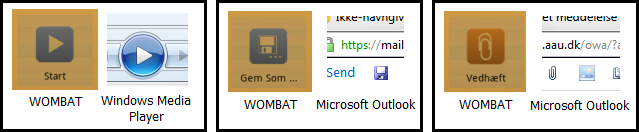
\includegraphics[width=\textwidth]{Images/Implementation/wombat_metaphors.png}
				\caption{Metaphors implemented in WOMBAT and the original implementation.}
		\label{fig:metaphors}
	\end{figure}